%%
%% This is file `mcmthesis-demo.tex',
%% generated with the docstrip utility.
%%
%% The original source files were:
%%
%% mcmthesis.dtx  (with options: `demo')
%%
%% -----------------------------------
%%
%% This is a generated file.
%%
%% Copyright (C)
%%     2010 -- 2015 by Zhaoli
%%     2014 -- 2016 by Liam 
%%     2017 -- 2019 by Xuehan
%%
%% This work may be distributed and/or modified under the
%% conditions of the LaTeX Project Public License, either version 1.3
%% of this license or (at your option) any later version.
%%
%% This work has the LPPL maintenance status `maintained'.
%%
%% The Current Maintainer of this work is Xuehan.
%%
\documentclass{mcmthesis}
\mcmsetup{CTeX = false,   % 使用 CTeX 套装时,设置为 true
        tcn = 2105529, problem = D,
        sheet = true, titleinsheet = true, keywordsinsheet = true,
		titlepage = true}
\usepackage{palatino}
\usepackage{mwe}
\usepackage{graphicx}
\usepackage{subcaption}
\usepackage{float}
\usepackage{multirow}
\usepackage{indentfirst}
\usepackage{gensymb}
\usepackage[ruled,lined,commentsnumbered]{algorithm2e}
\usepackage{diagbox}
\usepackage{enumerate}
\usepackage{tabu,adjustbox}
\usepackage[
natbib = true,  
backend=biber,  
% backend=bibtex,  
isbn=false,  
url=false,  
doi=false,  
eprint=false,  
style=numeric,  
% sorting=nyt,  
% sortcites = true
]{biblatex}
\usepackage{biblatex2bibitem}
\addbibresource{ref.bib}

\usepackage{geometry}
\geometry{left=2cm,right=2cm,top=2cm,bottom=2cm} %%页边距,若对左右边距进行修改,请保证左右边距一样,并且将mcmthesis.cls第81行对应的margin参数设置为相同数值
\begin{document}
\linespread{0.8} %%行间距
\setlength{\parskip}{0.7\baselineskip} %%段间距
\title{Figuring Out the Best Packaging Technique in Data Broadcasting}

\date{\today}
\begin{abstract}

	In complicated topologies, the choice of broadcasting patterns dominates the effectiveness of data transmission. The best strategy involves a combination of singlecasting and multicasting, which demands sophisticated packaging techniques. Therefore, it is vital to find the optimal algorithm for packaging branch information. In this paper, We make a very meaningful attempt to calculate the efficiency of different packaging strategies and compare them.

	There exists certain conditions where the optimal algorithm for packaging branch information can be discovered through pure reasoning. However, the best strategy in a certain topology system is not always apparent. Therefore, we decide to develop reasonable models to \textbf{quantify the efficiency} of different patterns. After that, we use enumeration to discover the optimum one.

	Primarily, we study certain topologies with certain pack capacities. We find that in cases like Task 1, the amount of receiving points and the minimum number of redundancy could be decided by \textbf{reasoning}.
	
	Then we study certain topologies with uncertain pack capacities. We find that, in order to reach a comprehensive optimum, we need to reach a \textbf{balance} between \textbf{the redundancy on edges} and \textbf{the loss of capacity caused by headers}. Therefore, we develop a model to \textbf{quantify} those losses and then compare them. Afterward, we \textbf{optimize the previous model} to fit in more complicated situations. We adopt both models in Task 2 and find the best strategy.
	
	Finally, we manage to find the optimal algorithm for packaging branch information. We achieve this by several steps. First, we simplify the topology by \textbf{aborting unconnected and unnecessary branches}. Second, we further \textbf{simplify the topology network to an array} and \textbf{describe it in two dimensions}. Third, we \textbf{modify our previous model} and \textbf{use the two dimensions to represent the function value}. Last of all, we use \textbf{heat map to enumerate different patterns and compare them in a visualized way}. 

	Now we are able to find the best strategy of packaging branch information. In the end, we discuss the advantage of our algorithm and draw a conclusion. 
	


	\begin{keywords}
		quantify, simplify to an array, heat map, enumerate, visualize
	\end{keywords}
\end{abstract}

\maketitle

\tableofcontents
\newpage

\section{Introduction}

\subsection{Problem Background}

Advancing towards a booming flow of information currents, the world is requiring more and more efficient broadcasting techniques to keep up the pace. Meanwhile, the number of Internet users is still under a sharp grow, making the topology blueprint even more sophisticated. As a result, there has been an urge to found the optimal pattern of information transmission.

Previous broadcasting involved the technique of unicast (or singlecast), by which only one pack of information is sent to one specific user at one time. Although its specific destination minimizes the capacity occupied by headers, this method would lead to great redundancy if the same pack needs to be sent to multiple users along the same path. We must appeal to a technique with greater efficiency in face with the rising transmission demand. Therefore, we need to find a balance between the capacity loss caused by headers and the redundancy of packs.

\subsection{Our work}
This paper aims to find a relatively optimal structure of a transmitting system. By investigating the combination of singlecasting and multicasting, we gradually gain insights into  and are able to develop an advanced

\section{Assumptions and Definitions}
\subsection{Our Assumptions}

We define \textbf{the length of the minimum path} from node U to node V as the \textbf{distance} between them. Then we make the following assumptions:
%Definition: a node u's distance from another node v: the length of the minimum path from u to v.

\begin{enumerate}[ \quad(1)]
	\item The topology is relatively balanced. Namely, the majority of nodes shares the same length of minimum path from the source and has an approximately equal amount of neighbors in the original topology.
	\item The complexity of the topology is directly proportional to its scale. The longer the minimum length from the source, the larger the amount of nodes.
	\item The topology is undirected. As long as data can be transferred from router A to router B, it can also be transferred backwards.
	\item The topology is connected. We ditch those nodes that are disconnected to the source.
	\item The loss caused by redundancy grows linearly rather than exponentially. It is directly proportional to the amount of loads on an edge.
	\item The effectiveness in the network is only related to the length of path a data packet covered and has nothing to do with the number of packets or the computing power of routers where packets are transferred.
	\item The transmitting network uses IP addresses to recognize different routers. We assume the global percentage of IPv6 is approximate to the percentage of IPv6 addresses visiting Google according to the statistical data given by Google, i.e. 32%.
	\item The weights of all edges are equivalent. Namely, the consumption is always the same when a same amount of data travels through a single edge.

\end{enumerate}


\subsection{Variable Definitions}
\begin{center}
	\begin{tabular}{cl}
		\hline
		Symbol  & Meaning                      \\
		\hline
		$f_{1}$ & a function describing redundancy \\
		$f_{2}$ & a better function                \\
		$f_{s}$ & a simpler function equivalent to $f_{2}$, only has the difference of constant                                \\
		$V_{i}$ & a node in the simplified network which has distance $i$ from the source                                 \\
		$N_{i}$ & the number of $V_{i}$ in the simplified network                                 \\
		$T_{i}$ & a tree structure in the simplified network which use $V_{i}$ as root                                  \\
		$S_{i}$ & the number of nodes in a single $T_{i}$                                 \\
		$U$     & the number of all users in the simplified network                                \\
		$I_{A}$ & the amount of information contained in the whole pack                                 \\
		$I_{H}$ & the amount of information contained in the head of the pack                                   \\
		$I_{G}$ & the amount of valid information contained in the pack                                  \\
		$n$     & the amount of $T_{i}$ contained in the header                                 \\
		$i$     & the rank of $T_{i}$ contained in the header                                 \\
		$N$     & the distance from the source to the furthest targeted point                                 \\
		$R$     & pure road redundancy                                 \\
		\hline
	\end{tabular}
\end{center}

\section{Topologies with Certain Packet Capacity -- Task 1}
\subsection{Calculating the maximum number of receiving points}

We study possible paths originating from node A. Since duplicate payloads are not allowed to appear, the data can only access node B C D once, respectively. Then we reach the next level of the question.

Given that the maximum number of branches on the header is 3, we know that the pack can get through at most 2 edges after reaching the second point. That means at most two other points can be reached.

However, there is only one edge (D-H) after node D, indicating that only one other point is available. As to node B and node C, the upper limit can both be reached.

Therefore, the number of receiving points cannot exceed 9. In detail, 3 for B and two other points, 3 for C and two other points, 2 for D and one other point and 1 for the source point A.

We can easily find a none-redundant distribution with 9 receiving points. The example is as follows:

\begin{figure}[H]
	\centering
	\includegraphics[width = 0.6\textwidth]{figure/fig.1-1.png}
	\caption{e.g.}
	\label{fig:1-1}
\end{figure}




\begin{enumerate}[ \quad(1).]
	\item A-B-E-F
	\item A-C-F-J
	\item A-D-H
\end{enumerate}

\subsection{Calculating the minimum number of redundancy}

Primarily, we discover that paths \textcolor[RGB]{180,76,151}{\bf{A-E-H-O}} and \textcolor[RGB]{230,176,112}{\bf{A-D-J-M}} are mandatory if we want all nodes to be reached. The reason is that, these two paths are the only approaches to get to node O and M -- All the other available paths cover more than 3 edges, which would violate the pack capacity.

Therefore, another two headers \textcolor[RGB]{91,126,145}{\bf{AE-EI-EL}} and header \textcolor[RGB]{222,108,141}{\bf{AC-CG-CK}} can be determined. Since nodes I and L can only be reached through edge A-E if we don't want to violate the maximum capacity, we adopt the former multicast header to keep the number of redundancy as small as possible. The same is with the latter.

Then we find that we need at least two single headers to get to node P, Q, N. The 3 nodes are all 2 edges away from the source, so multitasking can only reach 2 of 3. Apparently, the remaining node requires another singlecast to be covered. These, along with the mandatory path A-D-J-M demonstrated above, suggest that the minimum number of redundancy must be larger or equal to 3 in that edge A-D has already been traveled for 3 times.

We find such a pattern shown in the figure below

\begin{figure}[H]
	\centering
	\includegraphics[width = 0.6\textwidth]{figure/fig.1-2.png}
	\caption{e.g.}
	\label{fig:1-2}
\end{figure}

Thus, the minimum number of redundancy in this case is 3.


\section{Topologies with Uncertain Packet Capacity -- Task 2}

We try to figure out what makes a system relatively optimal. To do so, we investigate where and how superfluous information is generated. We discover two main sources of such information:

One is redundancy on the edges. Packets with the same payload may pass through the same edge multiple times, although in different headers. This leads to a loss of efficiency.

The other is the headers. They are also invalid information that reduce the actual capacity of the pack.

Therefore, to reach the optimum, we should find a balance between the two.

\subsection{Setting up an assessing model -- establishing $f_1$}

We define the following variables.

\begin{center}
	\begin{tabular}{cl}
		\hline
		Symbol  & Definition                                         \\
		\hline
		$I_{H}$ & The amount of header information in a certain pack \\
		$I_{A}$ & The amount of all information in a certain pack    \\
		$I_{G}$ & The amount of valid information in a certain pack  \\
		\hline
	\end{tabular}
\end{center}

\begin{description}
	\item [Note 1:] $I_{A}$ $I_{G}$ $I_{H}$ are all measured by how many users' information the whole pack / valid part / head part can hold, and differs from pack to pack.
	\item [Note 2:] The amount of equivalent redundancy include any node that is covered in a transmission path. In this specific task this doesn't matter, but we may need the declaration later on.
\end{description}

We establish the following formula:

\quad$f_1 = R+\frac{E*I_{H}}{I_{G}}$


where $f_1$ stands for the average number of edges that a receiving point utilizes to transmit one unit of valid information.



It can represent the efficiency of a system to a fair extent.

Based on the model, we are now able to calculate the degree of efficiency of a certain transmitting pattern. The minimum value of $f_1$ represents the most advanced pattern.

\subsection{Optimization of the present model -- establishing $f_2$}

However, we find that this model may not work well in certain complicated situations. On one hand, the model does not take into account whether the load of an edge changes from zero to one. But in real situations this change will also add to the consumption of the system. On the other hand, the model may suggest the pack go through unnecessarily long paths to avoid redundancy on a single edge. We have raised an example in the following topology to illustrate this.

THIS IS AN IMAGE (CUE QYH)

Consequently, we create another model to handle the dilemma.

%\quad\text{ $f_2$ = ( E * $I_{A}$ ) /( $I_{G}$ * $I_{H}$ ) }
We define the following variables.

\begin{center}
	\begin{tabular}{cl}
		\hline
		Symbol  & Definition                               \\
		\hline
		$E$     & The amount of utilized edges             \\
		$U$     & The amount of receiving nodes            \\
		$I_{A}$ & The scale of information per pack        \\
		$I_{G}$ & The scale of valid information per pack  \\
		$I_{H}$ & The scale of header information per pack \\
		\hline
	\end{tabular}
\end{center}

%\begin{flushright}
%	\begin{table}[htbp]
%	% \centeringin
%	% \footnotesize
%	
%	\everyrow{\hline}
%	\tabulinesep=1.2mm
%	
%	\begin{tabu}to\textwidth {|X[c]|X[1.5, l]|}
%		\rowfont[c]{} Dotation &  Definition\\
%		Dotation adfadfadfadf & Definition dafad adf dfa d afa df adf ad fa d\\
%	\end{tabu}
%	
%	\caption{Meaningful caption}
%	\label{T:my_table}
%	
%\end{table}
%\end{flushright}
\begin{description}
	\item[Note 1: ] $I_{A}$ $I_{G}$ $I_{H}$ are all measured by how many users' information the whole pack / valid part / head part can hold.
	\item[Note 2: ] The amount of receiving nodes include any node that is covered in a transmission path. In this specific task this doesn't matter, but we may need the declaration later on.
\end{description}

We establish the following formula:

\quad$f_{2} = \frac{I_{A} * E}{\sum I_{G} * I_{H}} * \frac{E}{U}$


where $f_{2}$ stands for the average number of edges that a receiving point utilizes to transmit one unit of valid information.


\subsection{Implementation of the models -- Path Enumeration}

No matter in $f_{1}$ or $f_{2}$, we can all easily find that a redundancy cost a lot. Because of this, we try to find a solution of no redundancy. Since there are only four points connected to A, at most four packs can be sent. When there are no pack contain more than five users' information, we can easily prove that at least one user would be travelled twice because of B and D. We find a 5-5-4-4 method. 
Or if we allow a package contains a header of 6 users' information, we can have a method of 6-4-4-3.


\begin{figure}[H]
	\centering
	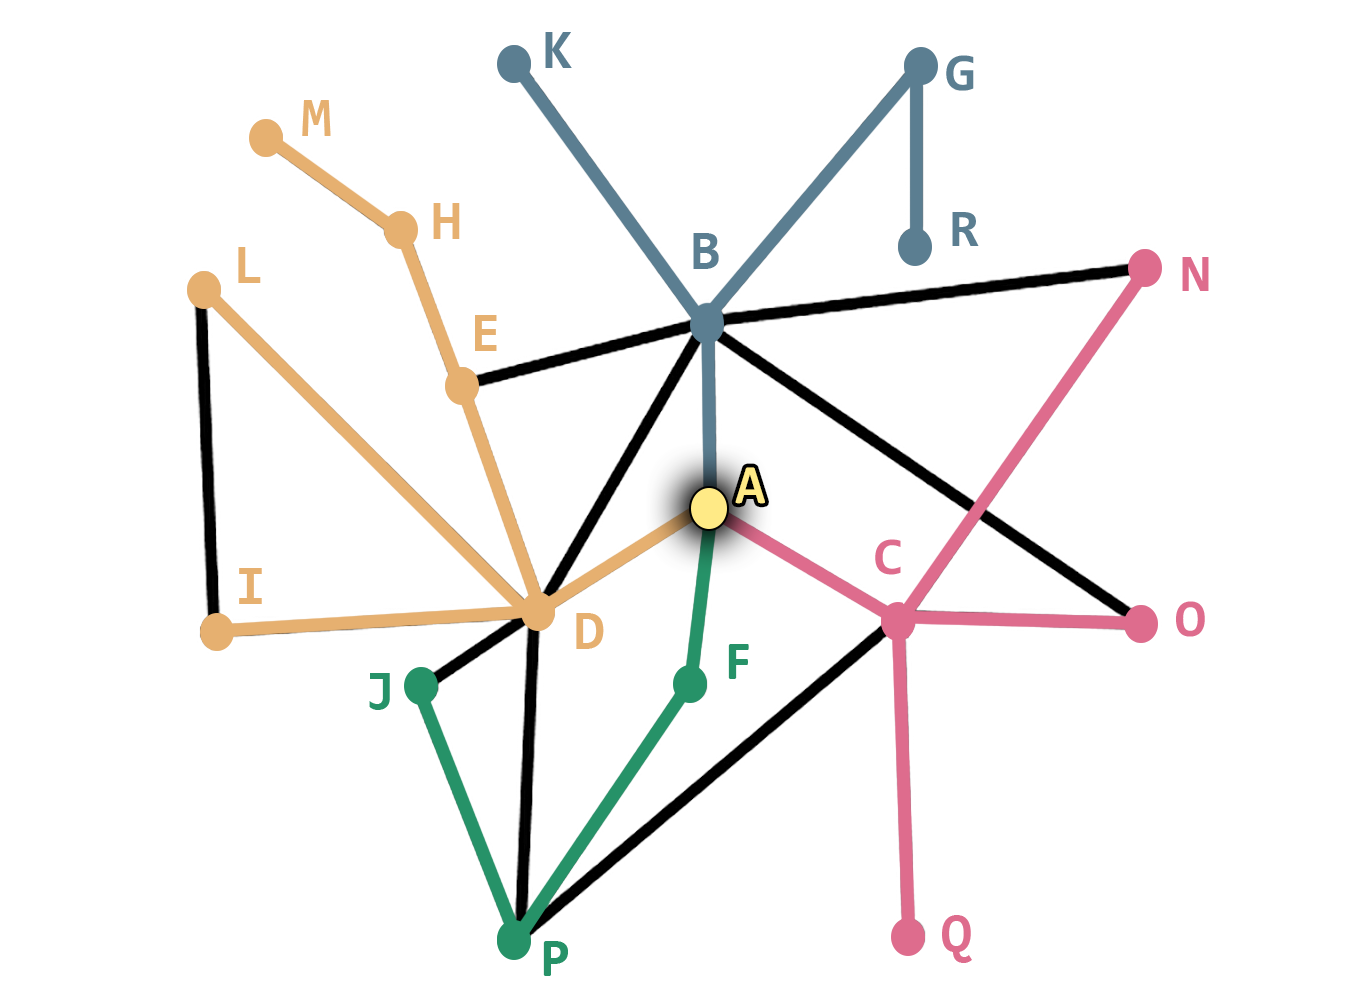
\includegraphics[width = 0.6\textwidth]{figure/6443.png}
	\caption{6443}
	\label{fig:1-2}
\end{figure}

\begin{figure}[H]
	\centering
	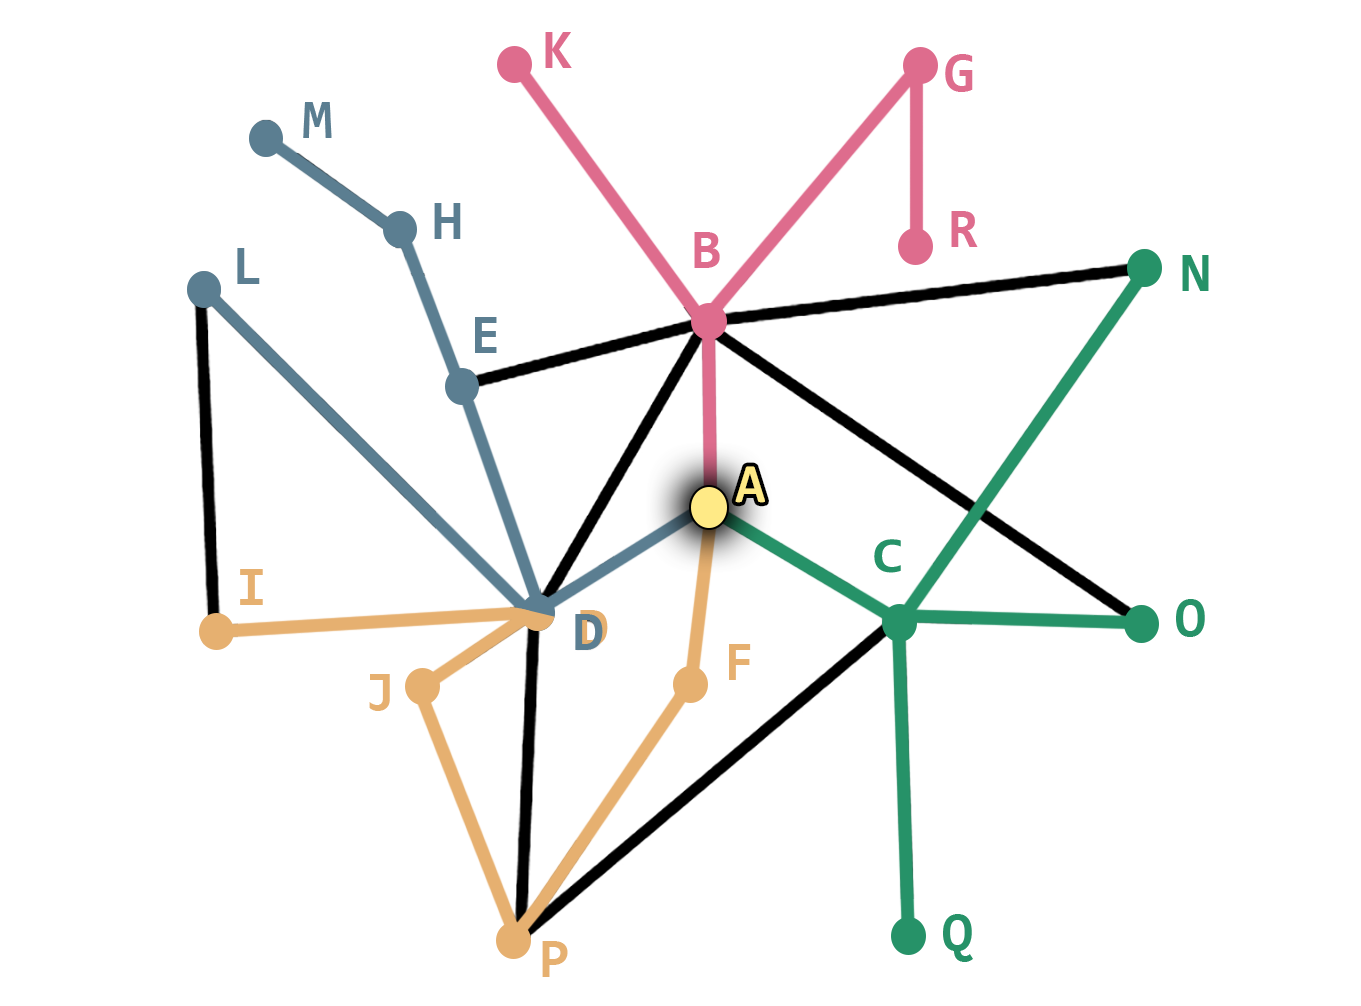
\includegraphics[width = 0.6\textwidth]{figure/5544.png}
	\caption{5544}
	\label{fig:1-2}
\end{figure}

After calculation, we find that the 6-4-4-3 strategy is better.

\section{Generalization to Topologies with Uncertain Packet Capacity -- Task 3}
\subsection{Reintroduction of our assessing models and their equalization}

In this part, we will reintroduce our problem. Given a network in reality, the only sender, and the many receivers, we want to find a good packaging strategy that can minimize information lost and
redundancy. To simplify the network, we will cut unnecessary edges and only focus on the necessary edges. Method is as follows. For each receiver, we find its shortest path to the sender, and whenever
it has multiple choices, we always choose the way that are less visited. Using this method, we got a nearly balanced network. That is to say, for each node having distance $i$ from the sender (called $V_{i}$),
they have the same status, and the simplified graph is a symmetrical tree where every node in it is receiver, and the root of the tree is the sender. Also, every node $V_{i}$ is a root to its child tree (called $T_{i}$),
because of the symmetry, each $V_{i}$ and $T_{i}$ are the same. We call the number of $V_{i}$ as $N_{i}$, and the number of nodes in $T_{i}$ as $S_{i}$. $N_{i}$ and $S_{i}$ are sequence that are only related to $i$.
Although the assumption seems rough, because of the law of big number, the model works surprisingly well. Also, since all the nodes become receivers, we can only focus on the point on the peek of the sequence $N_{i}$,
since if the peek of $N_{i}$ is covered, those nearer nodes are definitely covered, and for the further nodes, they are absorbed by the peek of $N_{i}$ in the formula, and they also do not have a high proportion. We use $i$ and $n$
to describe a packaging strategy, meaning a pack has the information of nodes in $n$ $T_{i}$. Using this model, we can give a dedicated calculation.

\subsection{Function calculation}

\begin{align}
    f_{s}(i,m) &=\frac{E}{I_{A}-I_{H}}     =\frac{N_{i}}{m} \cdot \frac{I_{H}}{I_{A}-I_{H}} \quad(\text{ since }  W=\frac{N_{i}}{m} I_{H}) \notag\\
    &=\frac{N_{i} S_{i}}{I_{A}+i-1-\left(I_{H}+\frac{I_{A}(i-1)}{I_{H}}\right)} \quad(\text{ since }   I_{H}=m S_{i} +i-1) \notag \\
    & \geqslant \frac{N_{i} S_{i}}{I_{A}-2 \sqrt{I_{A}(i-1)}+i-1} \label{ineq1}  \\
    & =\frac{N_{i}+\cdots+N_{n}}{\left(\sqrt{I_{A}} -\sqrt{i-1}\right)^{2}}, \notag
    \end{align}
    where the equality  in inequality \eqref{ineq1} holds if and only if 
	$\quad I_{H}=\sqrt{I_{A}(i-1)}$, namely,  $m=\frac{\sqrt{I_{A}(i-1)}-\left(i -1\right)}{S_{i}} $.
	$$
    \begin{aligned}
      f_{s}(i+1)-f_{s}(i)=&-\frac{N_{i}}{\left(\sqrt{I_{A}}-\sqrt{i}\right)^{2}}+\left(N_{i}+\cdots+N_{n}\right)\left(\frac{1}{\left(\sqrt{I_{A}}-\sqrt{i}\right)^{2}}-\frac{1}{\left(\sqrt{I_{A}}-\sqrt{i-1}\right)^{2}}\right)\\
      \approx &  \frac{1}{I_{A}}\left(-N_{i} \sqrt{i}+\frac{U}{\sqrt{I_{A}}}\right)
    \end{aligned}
    $$

	
In the step of finding the optimal $n$ and $i$, we also draw a graph.

The data we use comes from real data.


Also, we write a program that can transform network to arrays by breadth first search(BFS), try different $i$ and $n$, and draw the value of functions under different conditions.
 We can find that the result of the program is exactly the same with theoretical calculation. And the heat map conveys a good insight that what will occurs when $i$ and $n$ changes. 
 


 \begin{figure}[H]
	\centering
	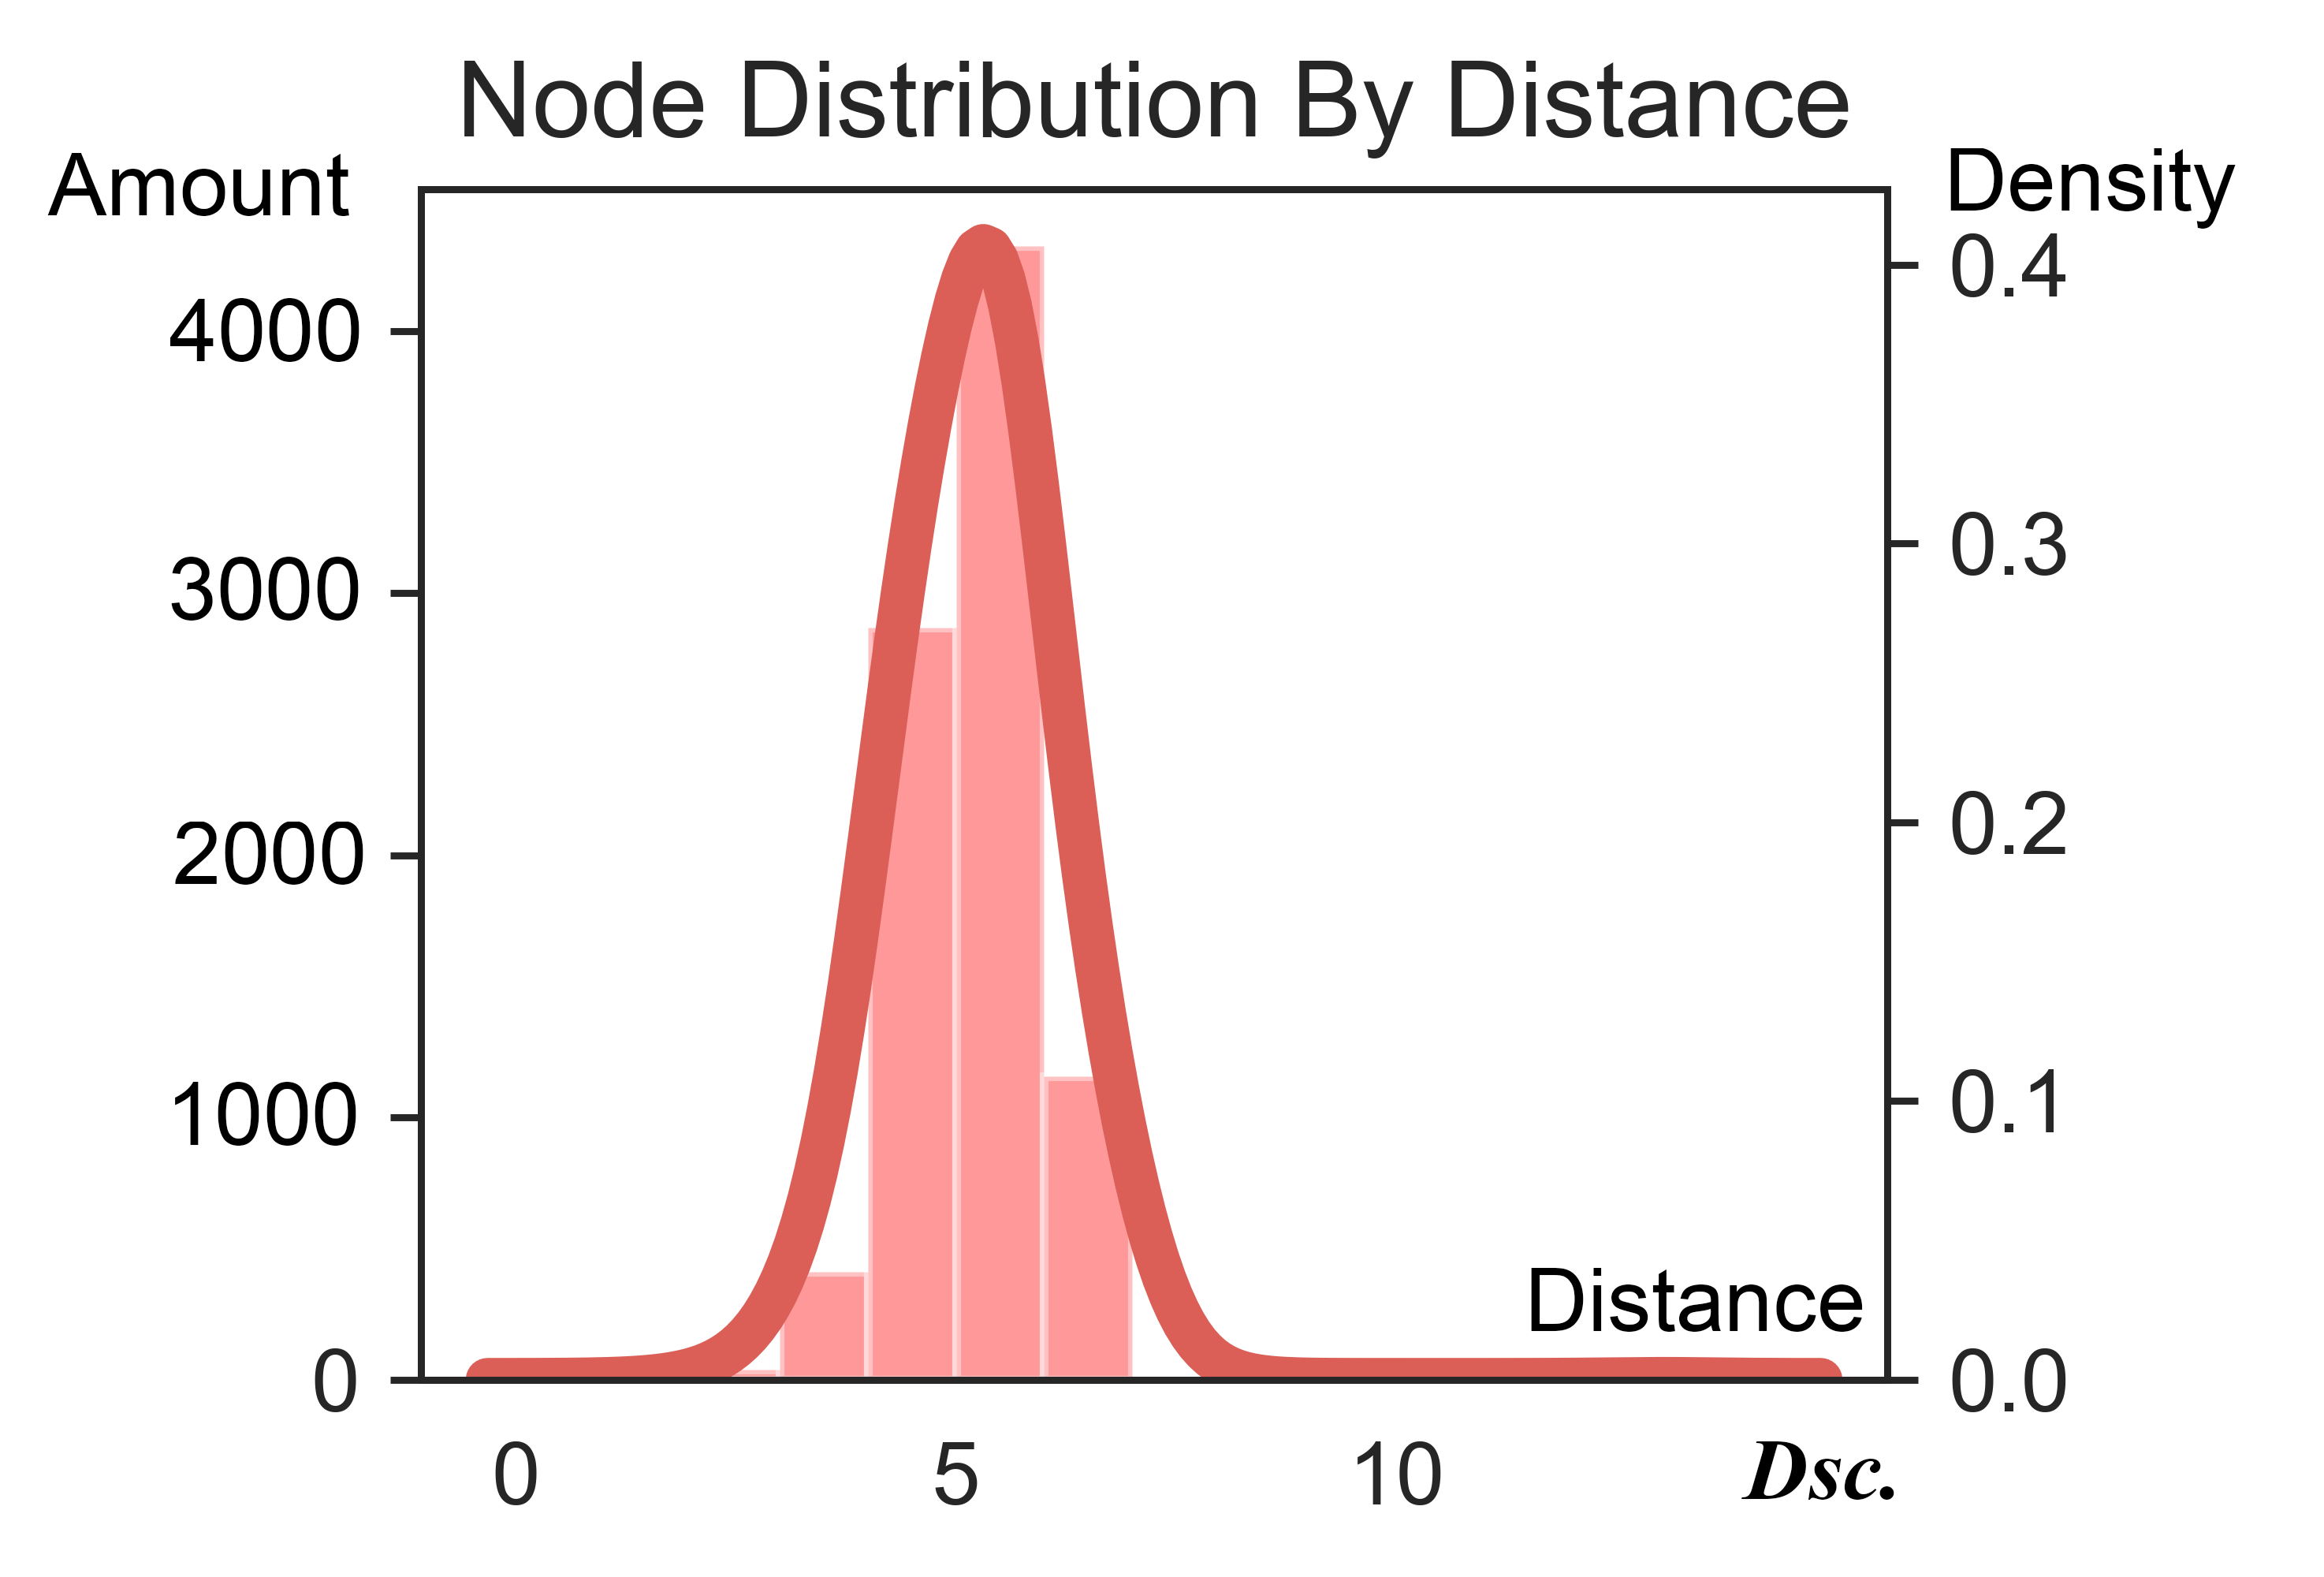
\includegraphics[width = 0.6\textwidth]{figure/hist06.png}
	\caption{distance distribution of nodes}
	\label{fig:1-1}
\end{figure}

 \begin{figure}[H]
	\centering
	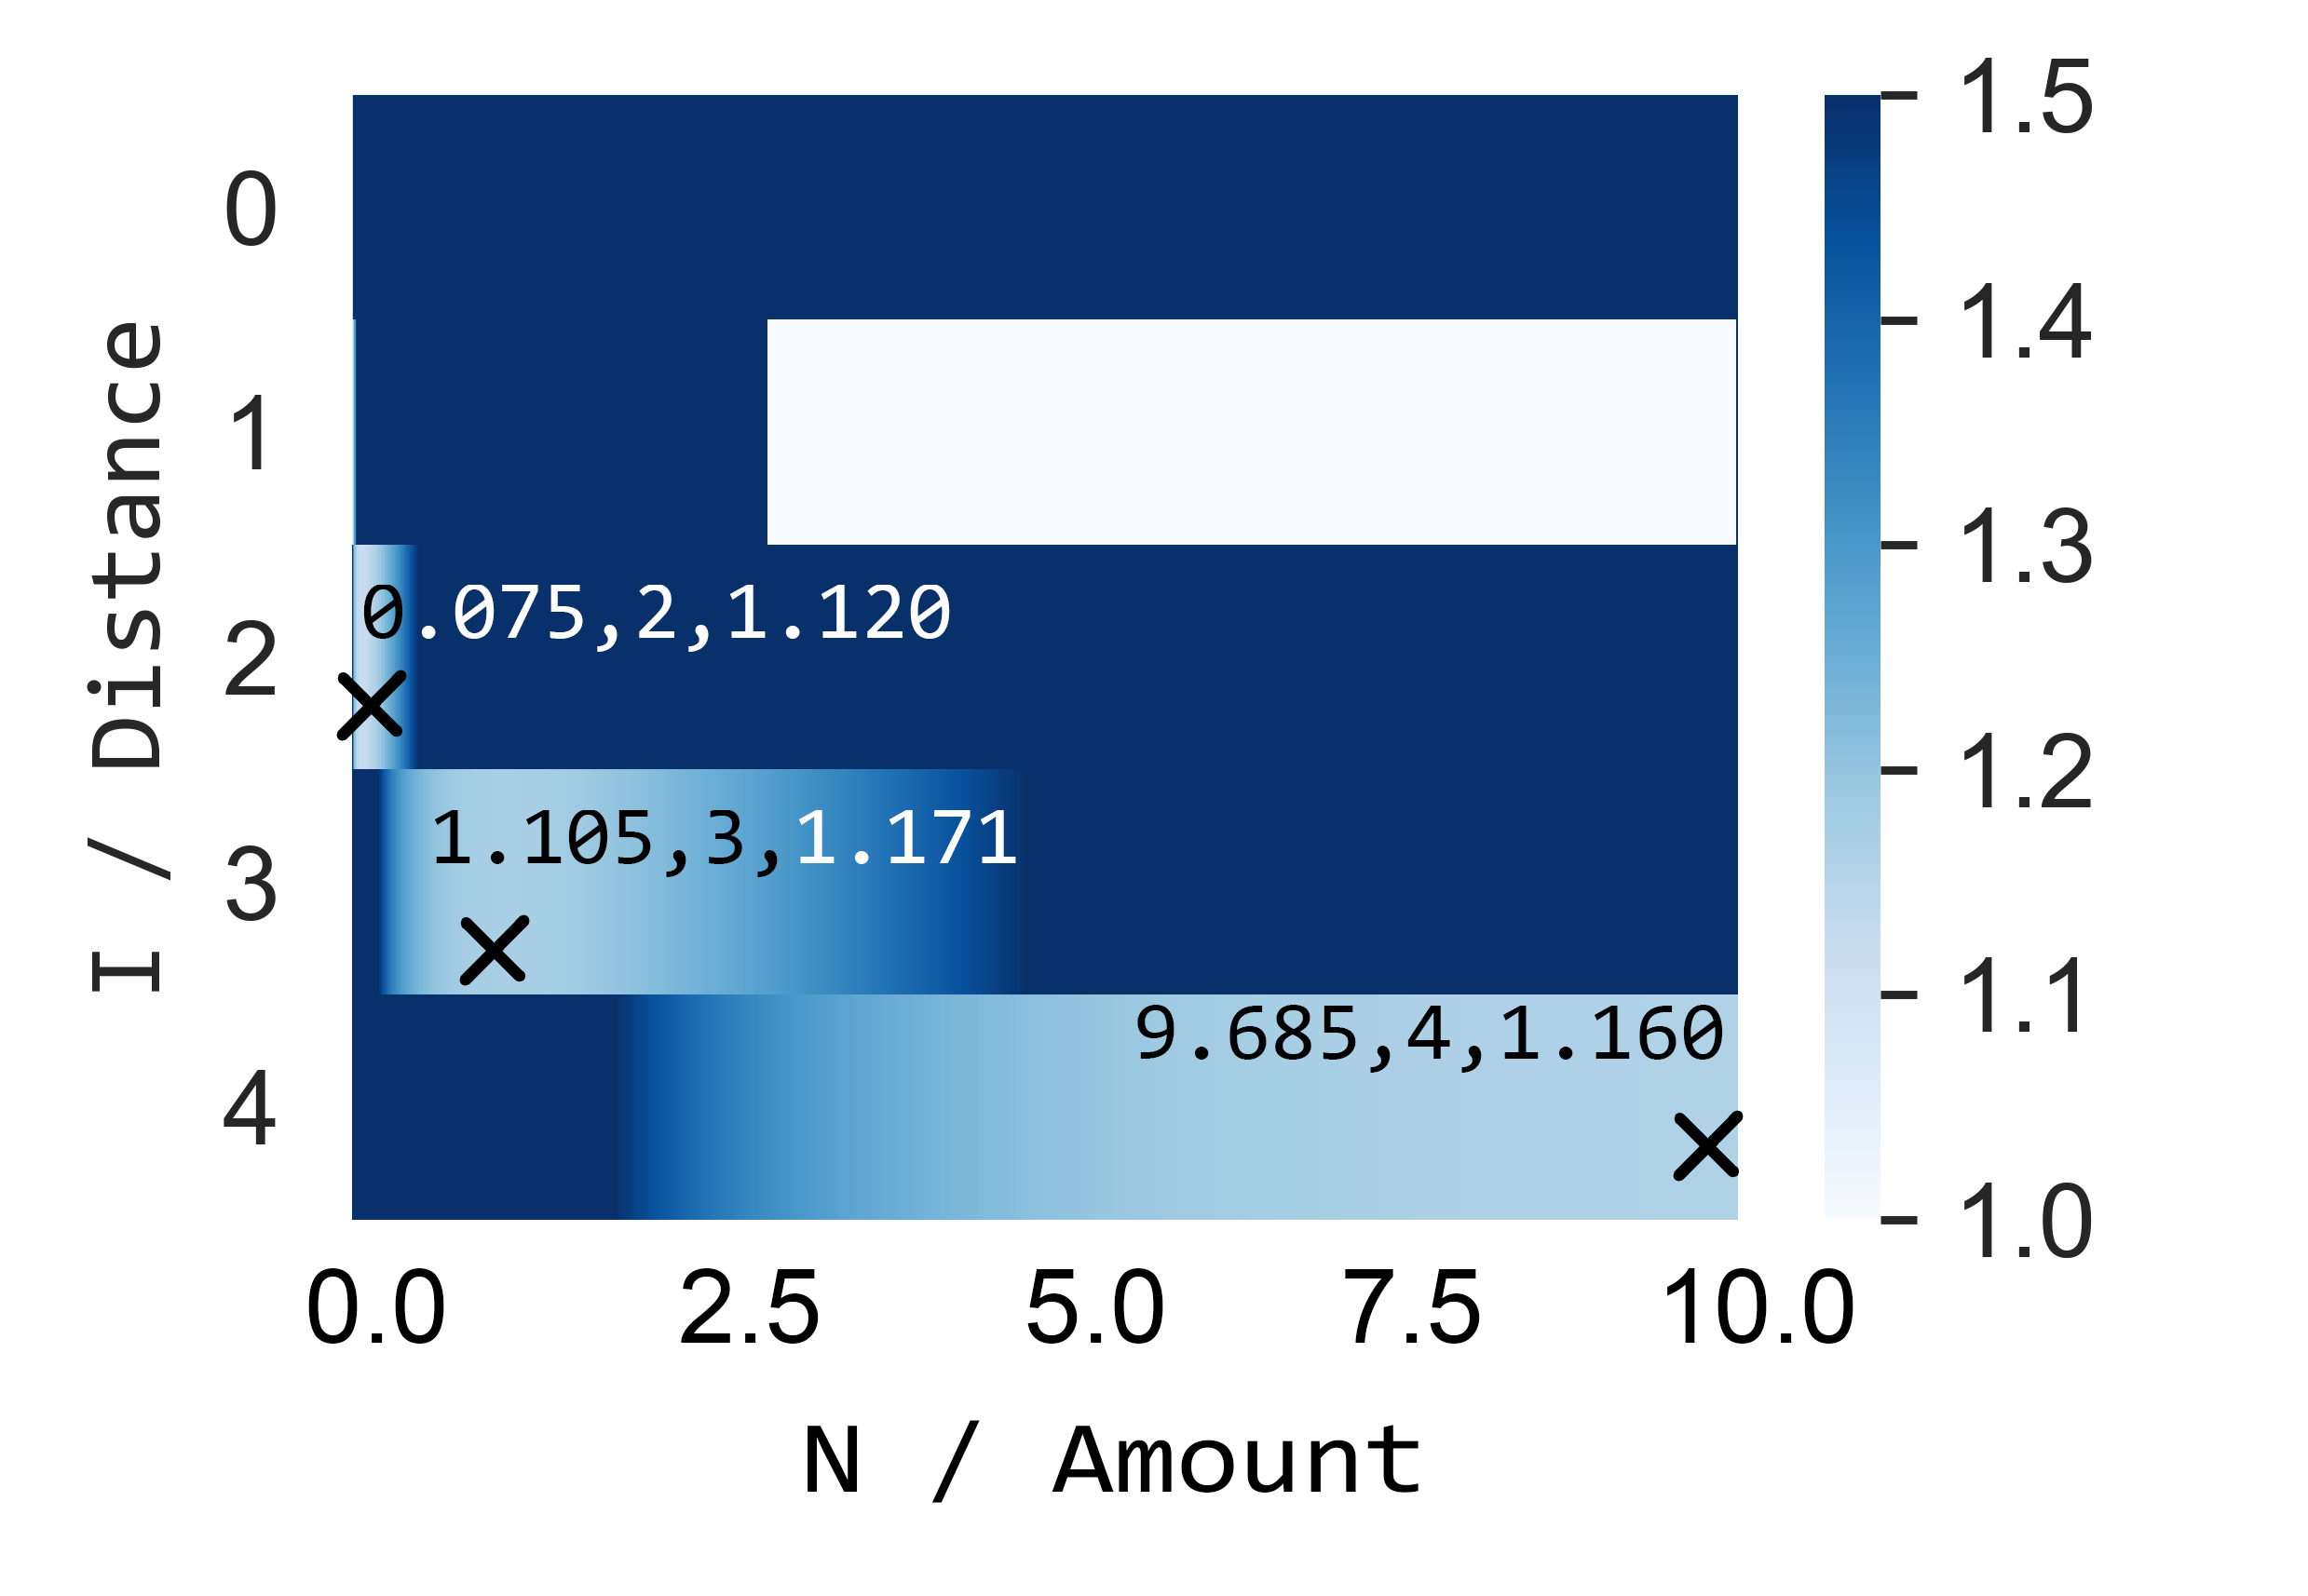
\includegraphics[width = 0.6\textwidth]{figure/Heapmap06.png}
	\caption{hot map showing the value of $f_{s}(i,n)$ and its minimum value}
	\label{fig:1-1}
\end{figure}







 Using this code and the Data in Text2 as an example, we calculated that it is the best when $i$ = 1 and $n$ = 1.1, or $i$ = 2 and $n$ = 2.5, and on both circumstances $f_{1}$ = 1.27,
 having 98\% of accuracy from the true value $f_{1}$ = 1.29! Also, using $i$ and $n$ as guides, we can easily know how much information the header should contain. As an example, in this case, 
 $i$ = 1 and $n$ = 1.1 means that each pack should solve one of its nearest road, which is exactly the case. Also in classic case like star graph, complete graph and linear graph, this algorithm also find the best solution.
 
%\begin{table}[H]
%	\centering
%	\caption{e.g}
%	\begin{tabular}{|c|c|c|}
%	\toprule
%	  & Symbol &Definition\\
%	\midrule
%	1 & 2 & 3\\	
%	1 & 2 & 3\\
%	1 & 2 & 3\\
%	1 & 2 & 3\\
%	1 & 2 & 3\\
%	\bottomrule
%	\end{tabular}
%	\label{tbl:eg1}
%\end{table}


\begin{table}[H]
	\centering
	\caption{e.g}
	\begin{tabular}{ccc}
		\hline
		\diagbox{a}{b}{c} & Symbol & Definition \\
		\hline
		1                 & 2      & 3          \\
		1                 & 2      &            \\
		1                 &        & 3          \\
		1                 & 2      & 3          \\
		                  &        & 3          \\
		\hline
	\end{tabular}
	\label{tbl:eg2}
\end{table}

%Example for Citation\cite{Jay_Rules}
%
%%\bibliographystyle{IEEETran}
%\bibliographystyle{plain}
%\bibliography{newrefs}

%\begin{center}
%	\begin{tabu} {|p{3cm}|X[l]|}
%		\addlinespace[1cm]
%		\multicolumn{2}{l}{ \textit{ [100]{bla bla} } } \\
%		\toprule
%		bla bla & bla bla bla bla bla bla bla bla \\
%		bla bla & bla bla bla bla bla bla bla bla \\
%		bla bla & bla bla bla bla bla bla bla bla \\
%		\bottomrule
%	\end{tabu}
%\end{center}

\section{Conclusion}

In this paper, we investigate the strategy of multicasting. First we use pure reasoning to solve Task1 which has fixed solution.
 Then we solved Task2 by both reasoning and function definition. We define a loss function called $f_{1}$ to show how much information are lost, and define another function called $f_{2}$ to show how much edge a user uses on average. The hardest part is Task3, where we build a model to solve the problem. In this model,
 we cut edges and simplified the network, compress the network to an array, setting different $i$ and $n$, using $i$ and $n$ to portray the evaluate function $f_{s}$, 
 use math skills to find the best solution of $i$ and $n$, find an extremely simple yet highly accurate way for human to decide how many information a header should contain, and program to
 visualize the result. Finally, we verified our result on simple graphs.

\newpage
%\cite*{snapnets}
%\cite*[PP. 531–-539]{MR1421568}
\nocite{*}



\printbibliography

% \bibliography{References}




% \printbibitembibliography


\begin{appendices}
	\section{The Code of Heat Map}
	\lstinputlisting[language=python]{code/ourcode.py}

\end{appendices}
\end{document}


%%%aaaaaaaaaaaaaaaaaaaaaaaaaaaaaaa